%----------------------------------------------------------------------------
\chapter{Összefoglalás}
%----------------------------------------------------------------------------

A szakdolgozat keretében megismerkedtem a Eclipse integrált fejlesztői környezettel, 
az Eclipse Modeling Framework technológiával, a EMF-IncQuery és a hozzá tartozó, lekérdezések szöveges leírására szolgáló nyelv használatával, és az Xtext validátorok írásával.
Elemeztem a nyelvben statikus analízis segítségével megoldható problémák témakörét, és kiválasztottam ezek közül egy gyakran előforduló és kellemetlen következményekkel járó problémát, melynek kezelése mégis egyszerű, \sout{a féléves munka során megvalósítható}.
A probléma okának és körülményeinek mélyebb megismerése után megterveztem és megvalósítottam a megoldáshoz szükséges ellenőrzést.
Az elkészült alkotást működés közben a ~\ref{fig:unusedLive}. ábra mutatja.
\sout{Ugyan éles bevetésére még nem került sor}, az EMF-IncQuery fejlesztői és felhasználói már most élénk érdeklődést mutatnak iránta.
\begin{figure}[h]
\centering
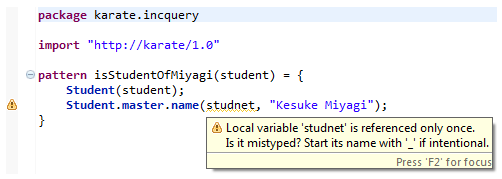
\includegraphics[width=0.85\textwidth]{figures/unused-variable-detection-warning.png}
\caption{Az elkészült ellenőrzés futás közben}
\label{fig:unusedLive}
\end{figure}

\section{Kitekintés}
A témához kapcsolódó további fejlesztések egyik lehetséges iránya a változók tí\-pu\-sá\-nak 
kikövetkeztetése, aminek segítségével további felhasználói mulasztások kerülhetőek el és akár a 
keresések optimalizálása is lehetővé válik.
